\chapter{Seitenlayout}

\lipsum[1]

\section{Satzspiegel}

Als \emph{Satzspiegel} wird der Bereich der Seite bezeichnet, auf dem der
eigentliche Text (siehe unten für Kopf- und Fußzeilen) stehen kann. Er wird
begrenzt durch die vier Seitenränder. Ziel ist es, den Satzspiegel so zu wählen,
dass er »harmonisch« wirkt.

\subsection{Klassische Buchdoppelseite}

Wir wollen dies zunächst am klassischen Beispiel eines Buches beschreiben. Ist
ein Buch aufgeschlagen, so sieht man eine \emph{linke} und eine \emph{rechte}
Seite. Da beiden Satzspiegel zueinander »am Buchsteg gespiegelt« ausgerichtet
sein sollen, ist es daher sinnvoll, die Seitenränder »oben«, »unten«, »innen«
und »außen« zu betrachten. Im strengen klassischen Buchsatz gelten folgende
Prinzipien:
\begin{enumerate}[nosep]
\item Der äußere Rand ist doppelt so groß wie der innere.
\item Der untere Rand ist doppelt so groß wie der obere.
\item Das Seitenverhältnis des Satzspiegels gleicht dem der Seite.
\end{enumerate}
Eine Umformulierung der vielleicht etwas willkürlich wirkenden ersten Regel ist,
das der \emph{gemeinsame} innere Rand genauso groß wie jeder der äußeren Ränder
ist. Befolgt man all diese Regeln, bleibt nur noch ein Freiheitsgrad übrig, und
dieser kann beschrieben werden durch das Breitenverhältnis zwischen Satzspiegel
und Seite. In \cref{fig:Satzspiegel} finden sich zwei Beispiele, wo dieses
Verhältnis einmal 70\,\% und einmal 60\,\% beträgt.

\begin{figure}
  \centering
  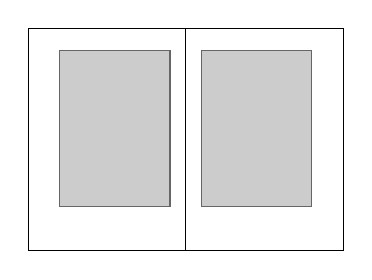
\begin{tikzpicture}[scale=2]
    \draw (0,0) rectangle (2,1.414);
    \draw (1,0) -- (1,1.414);
    \draw[black!60,thin,fill=black!20] (.2,.282) rectangle (.9,1.273);
    \draw[black!60,thin,fill=black!20] (1.1,.282) rectangle (1.8,1.273);
  \end{tikzpicture}\qquad
  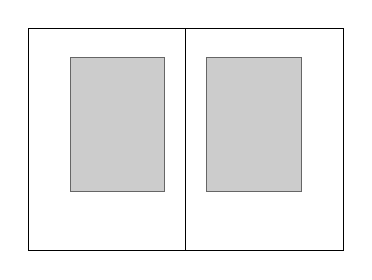
\begin{tikzpicture}[scale=2]
    \draw (0,0) rectangle (2,1.414);
    \draw (1,0) -- (1,1.414);
    \draw[black!60,thin,fill=black!20] (.267,.377) rectangle (.867,1.226);
    \draw[black!60,thin,fill=black!20] (1.133,.377) rectangle (1.733,1.226);
  \end{tikzpicture}
  \caption{Zwei Satzspiegel, die den klassischen Prinzipien genügen. Die
    Ausgangsseite hat (wie alle \acr{DIN}-Formate) ein Seitenverhältnis von
    1\,:\,$\sqrt{\text{2}}$. Das Breitenverhältnis zwischen Satzspiegel und Seite ist
    einmal 70\,\% (links) und einmal 60\,\% (rechts).}\label{fig:Satzspiegel}
\end{figure}

\subsection{Rasterteilung}

Anstatt dieses Breitenverhältnis anzugeben, wird in der Praxis der Satzspiegel
häufig durch \emph{Rasterteilung} bestimmt: Wir fixieren eine natürliche Zahl
$n$ und unterteilen die Seite gleichmäßig in $n$ Spalten und $n$ Zeilen. Nun
nehmen wir innen eine Spalte, außen zwei Spalten, oben eine Zeile und unten zwei
Zeilen weg; der verbleibende Bereich ist der Satzspiegel, siehe
\cref{fig:DIV}. Wir nennen $n$ den \emph{Rasterfaktor}. Auf diese
Weise sind nur noch Breitenverhältnisse der Form $\frac{n-3}{n}$ möglich. In
\LaTeX\ nimmt die \acr{KOMA}-Klasse \verb!scrbook! automatisch eine
Rasterteilung vor. Der Rasterfaktor kann z.\,B. durch \verb!DIV=9!
festgesetzt werden.

\begin{figure}
  \centering
  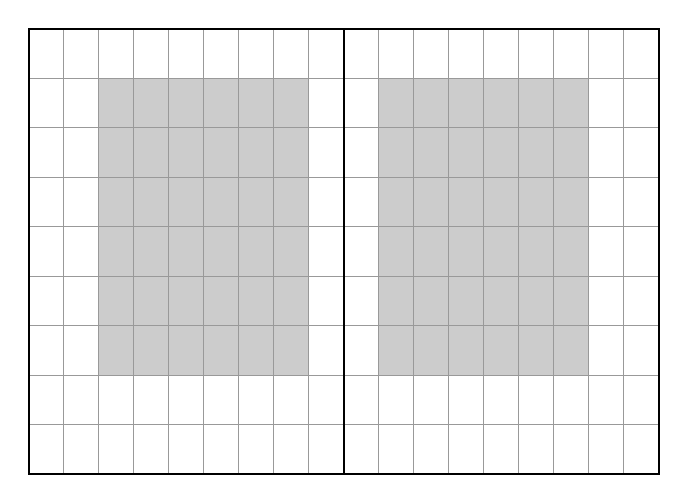
\begin{tikzpicture}[scale=4]
    \fill[black!20] ({2/9},{2*sqrt(2)/9}) rectangle ({8/9},{8*sqrt(2)/9});
    \fill[black!20] ({2-(2/9)},{2*sqrt(2)/9}) rectangle ({2-(8/9)},{8*sqrt(2)/9});
    \foreach \i in {1,...,8}{
      \draw[thin,black!40] ({\i/9},0) -- ({\i/9},{sqrt(2)});
      \draw[thin,black!40] (0,{\i*sqrt(2)/9}) -- (2,{\i*sqrt(2)/9});
      \draw[thin,black!40] ({(9+\i)/9},0) -- ({(9+\i)/9},{sqrt(2)});
    };
    \draw[thick] (0,0) rectangle (2,{sqrt(2)});
    \draw[thick] (1,0) -- (1,{sqrt(2)});
  \end{tikzpicture}
  \caption{Eine Rasterteilung mit Rasterfaktor 9, auch
    \emph{Neunerteilung} genannt. Das entstehende Breitenverhältnis ist
    \smallfrac69\,=\,\smallfrac23.}\label{fig:DIV}
\end{figure}

\subsection{Einseitiges Layout}

Im einseitigen Layout (geeignet für Dokumente, die nicht wie ein Buch
»aufgeklappt« werden) sind die Seitenränder links und rechts gleich groß; die
übrigen beiden Prinzipien gelten unverändert. Nicht ganz korrekterweise wird
auch hier der Begriff der \emph{Rasterteilung} verwendet, im Gegensatz zu obiger
Konstruktion werden allerdings nun links und rechts 1,5 Spalten entfernt, siehe
\cref{fig:einseitig}. So wird zum Beispiel von der \acr{KOMA}-Klasse
\verb!scrartcl! der Satzspiegel bestimmt.

\begin{figure}
  \centering
  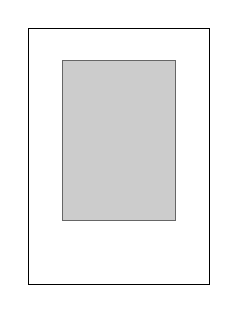
\begin{tikzpicture}[scale=2.3]
    \draw (0,0) rectangle (1,{sqrt(2)});
    \draw[black!60,thin,fill=black!20] (.1875,{.25*sqrt(2)}) rectangle (.8125,{.875*sqrt(2)});
  \end{tikzpicture}\quad
  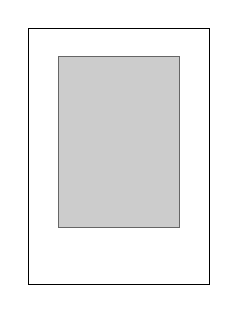
\begin{tikzpicture}[scale=2.3]
    \draw (0,0) rectangle (1,{sqrt(2)});
    \draw[black!60,thin,fill=black!20] (.167,{.222*sqrt(2)}) rectangle (.833,{.888*sqrt(2)});
  \end{tikzpicture}\quad
  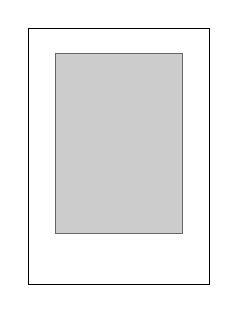
\begin{tikzpicture}[scale=2.3]
    \draw (0,0) rectangle (1,{sqrt(2)});
    \draw[black!60,thin,fill=black!20] (.15,{.2*sqrt(2)}) rectangle (.85,{.9*sqrt(2)});
  \end{tikzpicture}
  \caption{Mehrere einseitige Satzspiegel durch Rasterteilung, mit
    Rasterfaktor 8, 9 und 10.}\label{fig:einseitig}
\end{figure}

\subsection{Mehr Freiheit}

In moderneren Büchern wird das dritte Prinzip oft außer Acht gelassen. So ist
zum Beispiel dieses Skript für \acr{DIN-A5}-Papier gesetzt, d.\,h. die Seite hat
ein Verhältnis von 1\,:\,$\sqrt{\text{2}}$, während der Satzspiegel ein
Verhältnis von 3\,:\,5 hat. Ein Grund für diese Entwicklung ist vermutlich, dass
der untere Rand für zu groß befunden wurde.

\section{Zeilenlängen \emph{\&} Papierformate}

Nun stellt sich natürlich die Frage, nach welchen Kriterien das
Breitenverhältnis (bzw. der Rasterfaktor, der es am besten approximiert) gewählt
wird. Wieso nicht einfach 100\,\% (bzw. ein möglichst großer Rasterfaktor)? Die
entscheidende Einschränkung ist die \emph{Zeilenlänge}, die dadurch
quantifiziert wird, wie viele Zeichen des regulär formatierten Textes
durchschnittlich in eine Zeile passen. Konservative Typograph:innen empfehlen,
dass dieser Wert zwischen 60 und 80 Zeichen pro Zeile liegt, da ansonsten die
Lesbarkeit beeinträchtigt ist. Dieses Skript hat etwa 65 Zeichen pro Zeile. Je
nach Textgattung (etwa bei signifikantem Formelanteil) ist aber auch ein
größerer Wert geeignet. Wir weisen darauf hin, dass die Zeilenlänge von der
Laufweite der Schriftart abhängt.\todo{Laufweite in §3 erwähnen.}

Andererseits sollte natürlich auch noch ein relevanter Teil der Seite
beschreibbar sein. So sorgt ein Rasterfaktor von 7 zwar für kurze Zeilen,
allerdings wird am Ende auch nur \smallfrac{16}{49}, also etwa 32,6\,\% der
Seite bedruckt. Aus diesem Grund ist das Standardpapierformat \acr{DIN A4}
(210\,×\,297\,mm²) für die meisten Schriftstücke eigentlich zu groß, wie
\cref{tab:Papier} zeigt. Alternativen sind \acr{DIN B5} (176\,×\,250\,mm²) oder
\acr{DIN A5} (148\,×\,210\,mm²). Auf \acr{DIN A4} bietet sich hingegen ein
zweispaltiger Satz an; hier kann bei kurzer Zeilenlänge mehr Fläche bedruckt
werden.

\begin{table}
  \centering
  \begin{tabular}{rrrrr}
    \toprule
    \tableHead{Faktor} & \tableHead{Anteil} & \tableHead{DIN A4} & \tableHead{DIN B5} & \tableHead{DIN A5}\\
    \midrule
    \tab{11} & \tab{52,9}\,\% & \tab{100} & \tab{83} & \tab{72}\\
    \tab{10} & \tab{49,0}\,\% & \tab{96} & \tab{78} & \tab{68}\\
    \tab{9} & \tab{44,4}\,\% & \tab{90} & \tab{74} & \tab{64}\\
    \tab{8} & \tab{39,0}\,\% & \tab{85} & \tab{71} & \tab{61}\\
    \bottomrule
  \end{tabular}
  \caption{Anteil am Flächeninhalt und Zeilenlängen (für \acr{DIN A4}, \acr{DIN
      B5} und \acr{DIN A5}) für unterschiedliche Rasterfaktoren. Für dieses
    Experiment wurde die Schriftart Minion mit 11\,pt verwendet.}\label{tab:Papier}
\end{table}

\section{Kopf- und Fusszeilen}

\section{Blocksatz}

\section{Zeilenabstand}

\section{Umbrüche}


%% - Kopf-/Fußzeilen/Pagination
%% - Blocksatz, Silbentrennung
%% - Zeilenabstand
%% - Zeilen- und Seitenumbrüche
%% - Schriftgrößen mischen
%% - andere Formate (z.B. Plakate, Titelseiten, …)


%%% Local Variables:
%%% mode: latex
%%% TeX-master: "main"
%%% End:
